\input{configTD}


\title{Probabilités TD4 - Lois Normales et Intervalles de confiance}

\author{}
\date{}


\begin{document}
\sffamily
\maketitle

\section*{La loi normale}
On note $\Phi$ la fonction de répartion de la loi normale centrée réduite et on donne à la fin de ce TD la table de la loi normale centrée réduite. 
\begin{enumerate}
    \item Calculer $\Phi(1.96)$, $\Phi(2.58)$, $\Phi(-1.96)$, $\Phi(-2.58)$. 
    \ifthenelse{\boolean{showSolutions}}{
        \begin{solution}
            On lit les valeurs dans la table. 
            Pour la première valeur, on cherche $1.9$ en ligne et $0.06$ en colonne, on obtient $0.975$. 
            $\Phi(1.96) = 0.975$, 
            
            
            $\Phi(2.58) = 0.995$, $\Phi(-1.96) = 1- 0.975 = 0.025$, $\Phi(-2.58) = 1- 0.995 = 0.005$. 
        \end{solution}
    }{}
    \item Donner la probabilité qu'une loi normale centrée réduite soit supérieure à 1.96, puis qu'elle soit supérieure à 2.58. 
    \ifthenelse{\boolean{showSolutions}}{
        \begin{solution}
            La table donne aussi les valeurs : si $X$ suit une loi normale centrée réduite, alors 
            \[
            P(X < t) = \Phi(t)
            \]
            On en déduit que : 
            $P(X > 1.96) = 1- \Phi(1.96) = 0.025$, 
            
            $P(X > 2.58) = 1- \Phi(2.58) = 0.005$. 
        \end{solution}
    }{}
    \item Donner la probabilité qu'une loi normale centrée réduite soit comprise dans l'intervalle $[-1.96, 1.96]$, puis dans l'intervalle $[-2.58, 2.58]$. 
    \ifthenelse{\boolean{showSolutions}}{
        \begin{solution}
            $P(-1.96 < X < 1.96) = \Phi(1.96) - \Phi(-1.96) = 0.95$, 
            
            $P(-2.58 < X < 2.58) = \Phi(2.58) - \Phi(-2.58) = 0.99$. 
        \end{solution}
    }{}
\end{enumerate}

   On rappelle que si $X$ suit une loi normale $\mathcal{N}(m, \sigma^2)$, alors $Z = \frac{X - m}{\sigma}$ suit une loi normale centrée réduite. 
   On considère une variable aléatoire $X$ qui suit une loi normale $\mathcal{N}(10, 4)$. 
   \begin{enumerate}
    \item Calculer la probabilité que $X$ soit supérieure à 12. 
    \ifthenelse{\boolean{showSolutions}}{
        \begin{solution}
            $P(X > 12) = 1 - P(X < 12) = 1 - P\left(\frac{X-10}{2} < \frac{12-10}{2}\right) = 1 - \Phi(1) = 1 - 0.8413 = 0.1587$. 
        \end{solution}
    }{}
    \item Calculer la probabilité que $X$ soit comprise dans l'intervalle $[8, 12]$, puis dans l'intervalle $[6, 14]$.
    \ifthenelse{\boolean{showSolutions}}{
        \begin{solution}
            Pour le premier intervalle, on a : 
            \[P(8 < X < 12) = P\left(\frac{8-10}{2} < \frac{X-10}{2} < \frac{12-10}{2}\right) = \Phi(1) - \Phi(-1) = 0.8413 - 0.1587 = 0.6826.\] 
        
        Pour le second intervalle, on a : 
        \[P(6 < X < 14) = P\left(\frac{6-10}{2} < \frac{X-10}{2} < \frac{14-10}{2}\right) = \Phi(2) - \Phi(-2) = 0.9772 - 0.0228 = 0.9544.\] 
        \end{solution}
    }{}
   \end{enumerate}

   
   \vspace{0.1cm}

   \section*{Appliquer le théorème central limite}


On rappelle le \textbf{théorème central limite} : 
Si des variables aléatoires $X_1, X_2, \cdots, X_n$ sont indépendantes et de même loi telles que $E(X_1) = m$ et $\text{Var}(X_1) = \sigma^2$ existent, 
Alors la loi de la variable aléatoire 
$$S_n = \frac{\sqrt{n}}{\sqrt{\sigma^2}} \, \bigg(\frac{X_1 + X_2 + \cdots + X_n}{n} - m\bigg)$$ 
converge vers la loi normale centrée réduite. 


    On récolte des tomates dont le poids est le suivant : 
\begin{table}[h]
    \centering
    \begin{tabular}{|c|c|c|c|c|}
        \hline
        \textbf{Poids (g)} & 160 & 170 & 190 & 210 \\
        \hline
        \textbf{Nombre de tomates} & 20 & 25 & 30 & 25 \\
        \hline
    \end{tabular}
\end{table}

    On modélise le poids des tomates par une loi normale de moyenne inconnue $\mu$ et d'écart type $\sigma = 40$. 
    \begin{enumerate}
    \item Donner une estimation de $\mu$ à partir de la table de fréquence. 
    \ifthenelse{\boolean{showSolutions}}{
    \begin{solution}
        La somme des effectifs est $20 + 25 + 30 + 25 = 100$. On calcule la moyenne empirique : 
        \[
        \bar{X} = \frac{160 \times 20 + 170 \times 25 + 190 \times 30 + 210 \times 25}{100} = 184.
        \] 
        On en déduit une estimation de $\mu$ : $\hat{\mu} = 184$.
    \end{solution}
    }{}
    \item En appliquant le théorème central limite, donner un intervalle de confiance à 95\% pour $\mu$ centré autour de l'estimation précédente. 
    \ifthenelse{\boolean{showSolutions}}{
        \begin{solution}
            Le théorème donne : 
            \[
            \frac{\sqrt{n}}{\sqrt{\sigma^2}} \, \big(\hat{\mu} - \mu\big) \sim \mathcal{N}(0, 1)
            \]
        D'après l'exercice précédent, on sait qu'une loi normale centrée réduite est comprise entre $-1.96$ et $1.96$ avec une probabilité de $0.95$:
        \[
        P\bigg(\frac{\sqrt{n}}{\sqrt{\sigma^2}} \, \big(\hat{\mu} - \mu\big) \in [-1.96, \, 1.96]\bigg) = 0.95
        \] 
        On en déduit un intervalle de confiance à 95\% pour $\mu$ : 
        \[
        P\bigg(\mu \in \left[\hat{\mu} - 1.96 \frac{\sigma}{\sqrt{n}},\,  \hat{\mu} + 1.96 \frac{\sigma}{\sqrt{n}}\right]\bigg) = 0.95
        \] 
        En remplaçant $n$ par $100$ et $\sigma$ par $40$, on obtient : 
        \[
        P\bigg(\mu \in \left[184 - 1.96 \frac{40}{\sqrt{100}}, 184 + 1.96 \frac{40}{\sqrt{100}}\right]\bigg) = 0.95
        \] 
        On en déduit que : 
            \[
            \mu \in \left[176.16,\,  191.84\right]
            \] 
            avec une probabilité de $0.95$. 
        \end{solution}
    }{}
    \item Le vendeur de graines annonçait une récolte suivant une loi $\mathcal{N}(210, 40^2)$. 
    Si l'hypothèse du vendeur est correcte, quelle est la probabilité d'avoir obtenu une moyenne de récolte inférieure à celle que vous avez obtenue à la question précédente ?

    \textbf{Remarque : } Si $X_1$ et $X_2$ sont deux variables aléatoires indépendantes de loi $\mathcal{N}(m, \sigma^2)$, la variable aléatoire $\lambda X_1 + \mu X_2$ suit une loi $\mathcal{N}(\lambda m + \mu m, \lambda^2 \sigma^2 + \mu^2 \sigma^2)$. 
    \ifthenelse{\boolean{showSolutions}}{
        \begin{solution}
            Si l'hypothèse du vendeur est correcte, quelle loi devrait suivre la variable aléatoire $\hat{\mu}$ ? 
            On a $\hat{\mu} = \frac{X_1 + X_2 + \cdots + X_n}{n}$ où les $X_i$ sont des variables aléatoires de loi $\mathcal{N}(210, 40^2)$. 

            D'après la remarque, on en déduit que $\hat{\mu}$ suit une loi $\mathcal{N}\left(210, \frac{40^2}{n}\right)$. 
            La probabilité que cette variable aléatoire prenne la valeur $184$ ou moins est : 
            \[
            P\big(\hat{\mu} < 184\big) = \Phi\left(\frac{184 - 210}{\frac{40}{\sqrt{n}}}\right) = \Phi(-6.5) = 0.
            \] 
        \end{solution}
    }{}
    \item A quel point croyez-vous aux données du vendeur ? 
    \ifthenelse{\boolean{showSolutions}}{
        \begin{solution}
            La probabilité que $\hat{\mu}$ soit inférieure à $184$ est quasiment nulle $0$. Si l'hypothèse du vendeur était correcte, nous avons assisté à un événement très rare. 
            Nous pouvons donc raisonnablement rejeter l'hypothèse du vendeur. 
        \end{solution}
    }{}
   \end{enumerate}

   \vspace{0.1cm}

\section*{Pour des sondages}
On sonde $n$ électeurs au sujet d'une élection avec $3$ candidats $A$, $B$ et $C$. \newline
Sur les $n = 1000$ électeurs interrogés, $X = 300$ personnes déclarent qu'elles voteront pour le candidat~A.

\begin{enumerate}
    \item Déterminer l'estimation ponctuelle $\hat{p}$ de la proportion de votes en faveur du candidat A.
    \ifthenelse{\boolean{showSolutions}}{
        \begin{solution}
            Il suffit de faire le ratio du nombre de personnes qui ont voté pour $A$ sur le nombre total d'électeurs interrogés : 
            \[
            \hat{p} = \frac{X}{n} = \frac{300}{1000} = 0.3
            \] 
        \end{solution}
    }{}
    \item Calculer un intervalle de confiance à 95\% pour la proportion $p$. 
    \ifthenelse{\boolean{showSolutions}}{
        \begin{solution}
            Le théorème central limite donne : 
            \[
            \frac{\hat{p} - p}{\sqrt{\frac{p(1-p)}{n}}} \sim \mathcal{N}(0, 1)
            \]
            
            On prend le même intervalle que dans l'exercice précédent: $[-1.96, 1.96]$. 

            
            On en déduit que : 
            \[
                \frac{\hat{p} - p}{\sqrt{\frac{p(1-p)}{n}}} \in [-1.96, 1.96] \text{ avec une probabilité de } 0.95
            \]
            
            \[
                \hat{p} - p \in [-1.96 \frac{\sqrt{p(1-p)}}{\sqrt{n}}, 1.96 \frac{\sqrt{p(1-p)}}{\sqrt{n}}] \text{ avec une probabilité de } 0.95
            \]
            Ici, on a plusieurs solutions pour gérer le $p$ dans l'intervalle : 
            \begin{itemize}
                \item On peut remplacer $p$ par $\hat{p}$ et faire comme si de rien n'était. Ce n'est pas très rigoureux mais c'est une approche courante. 
                \item On peut majorer $p(1-p)$ par $\frac{1}{4}$. On obtiendra un intervalle un peu plus grand, mais on reste rigoureux mathématiquement. 
            \end{itemize}

            Quelle que soit l'option choisie, on obtient presque le même intervalle.  

            Continuons avec la seconde option :
            \[
                \hat{p} - p \in [ \frac{-1.96}{\sqrt{4n}}, \frac{1.96}{\sqrt{4n}}] \text{ avec une probabilité de } 0.95
            \]
            et donc 
            \[
                p \in \left[\hat{p} - \frac{1.96}{\sqrt{4n}}, \hat{p} + \frac{1.96}{\sqrt{4n}}\right] \text{ avec une probabilité de } 0.95
            \]
        
            On en déduit l'intervalle de confiance avec les valeurs numériques :
            \[
                p \in \left[0.3 - \frac{1.96}{\sqrt{4000}}, 0.3 + \frac{1.96}{\sqrt{4000}}\right] \text{ avec une probabilité de } 0.95
            \]
            On en déduit que : 
            \[
                p \in [0.269, 0.331] \text{ avec une probabilité de } 0.95
            \]
        \end{solution}
    }{}
    \item L'intervalle contient-il la valeur correspondant à un partage égal des votes ? 
    Que signifie ce résultat en termes d'incertitude sur l'élection ?
    \ifthenelse{\boolean{showSolutions}}{
        \begin{solution}
            Non, l'intervalle de confiance ne contient pas $0.3333333$, 
            il y a donc moins de $5\%$ de chances que la proportion de votes pour $A$ soit égale à $0.3333333$. 
        \end{solution}
    }{}
\end{enumerate}

\vspace{1cm}



\section*{Théorème central limite avec une autre loi}
   Un centre d'appels souhaite comparer la durée des appels de deux de ses salariés, Alice et Bob. 
On a relevé la durée de 60 appels pour chacun d'entre eux :

\begin{table}[h]
    \centering
    \begin{tabular}{|c|c|c|c|c|}
        \hline
        \textbf{Durée (minutes)} & 2 & 5 & 8 & 12 \\
        \hline
        \textbf{Nombre d'appels d'Alice} & 15 & 25 & 12 & 8 \\
        \hline
        \textbf{Nombre d'appels de Bob} & 8 & 14 & 23 & 15 \\
        \hline
    \end{tabular}
\end{table}

\begin{enumerate}
    \item Calculer la durée moyenne des appels pour chaque salarié.
    \ifthenelse{\boolean{showSolutions}}{
        \begin{solution}
            Pour Alice : \(\bar X_A = \frac{2\times15 + 5\times25 + 8\times12 + 12\times8}{60} = \frac{347}{60} = 5.78\text{ min}.\)
            
            \vspace{0.5cm}

            Pour Bob : \(\bar X_B = \frac{2\times8 + 5\times14 + 8\times23 + 12\times15}{60} = \frac{450}{60} = 7.5\text{ min}.\)
        \end{solution}
    }{}
    \item Par quelle loi classique peut-on modéliser la durée d'un appel pour chaque salarié ?
    \ifthenelse{\boolean{showSolutions}}{
        \begin{solution}
            La durée des appels est généralement modélisée par une loi exponentielle. 
        \end{solution}
    }{}
    \item Estimer les paramètres de ces lois à partir des données.
    \ifthenelse{\boolean{showSolutions}}{
        \begin{solution}
            On se rappelle que l'espérance d'une loi exponentielle est l'inverse de son paramètre. 
            On en déduit : 
            \[
            \hat\lambda_A = \frac{1}{\bar X_A} \approx \frac{1}{5.78} \approx 0.173, \quad \hat\lambda_B = \frac{1}{\bar X_B} = \frac{1}{7.5} \approx 0.133.
            \]
        \end{solution}
    }{}
    \item Le superviseur souhaite que la durée moyenne des appels soit inférieure à 6 minutes. L'un des deux salariés respecte-t-il cet objectif ?
    \ifthenelse{\boolean{showSolutions}}{
        \begin{solution}
            Alice a une moyenne \(\approx5.78<6\), elle respecte l'objectif. Bob a \(\bar X_B=7.5>6\), il ne le respecte pas.
        \end{solution}
    }{}
\end{enumerate}

\vspace{1cm}
\section*{Estimer une proportion}
Soit $X$ une variable aléatoire suivant une loi normale centrée réduite.
\begin{enumerate}
    \item Faite un dessin pour illustrer le fait que pour $\alpha \in] 0,1\left[\right.$, il existe un unique réel positif $t_\alpha$ tel que 
    \[P\left(-t_\alpha < X < t_\alpha\right)=1-\alpha.\]
    \ifthenelse{\boolean{showSolutions}}{
        \begin{solution}
            On trace la densité de la loi normale centrée réduite, symétrique par rapport à 0,
            \begin{center} 
                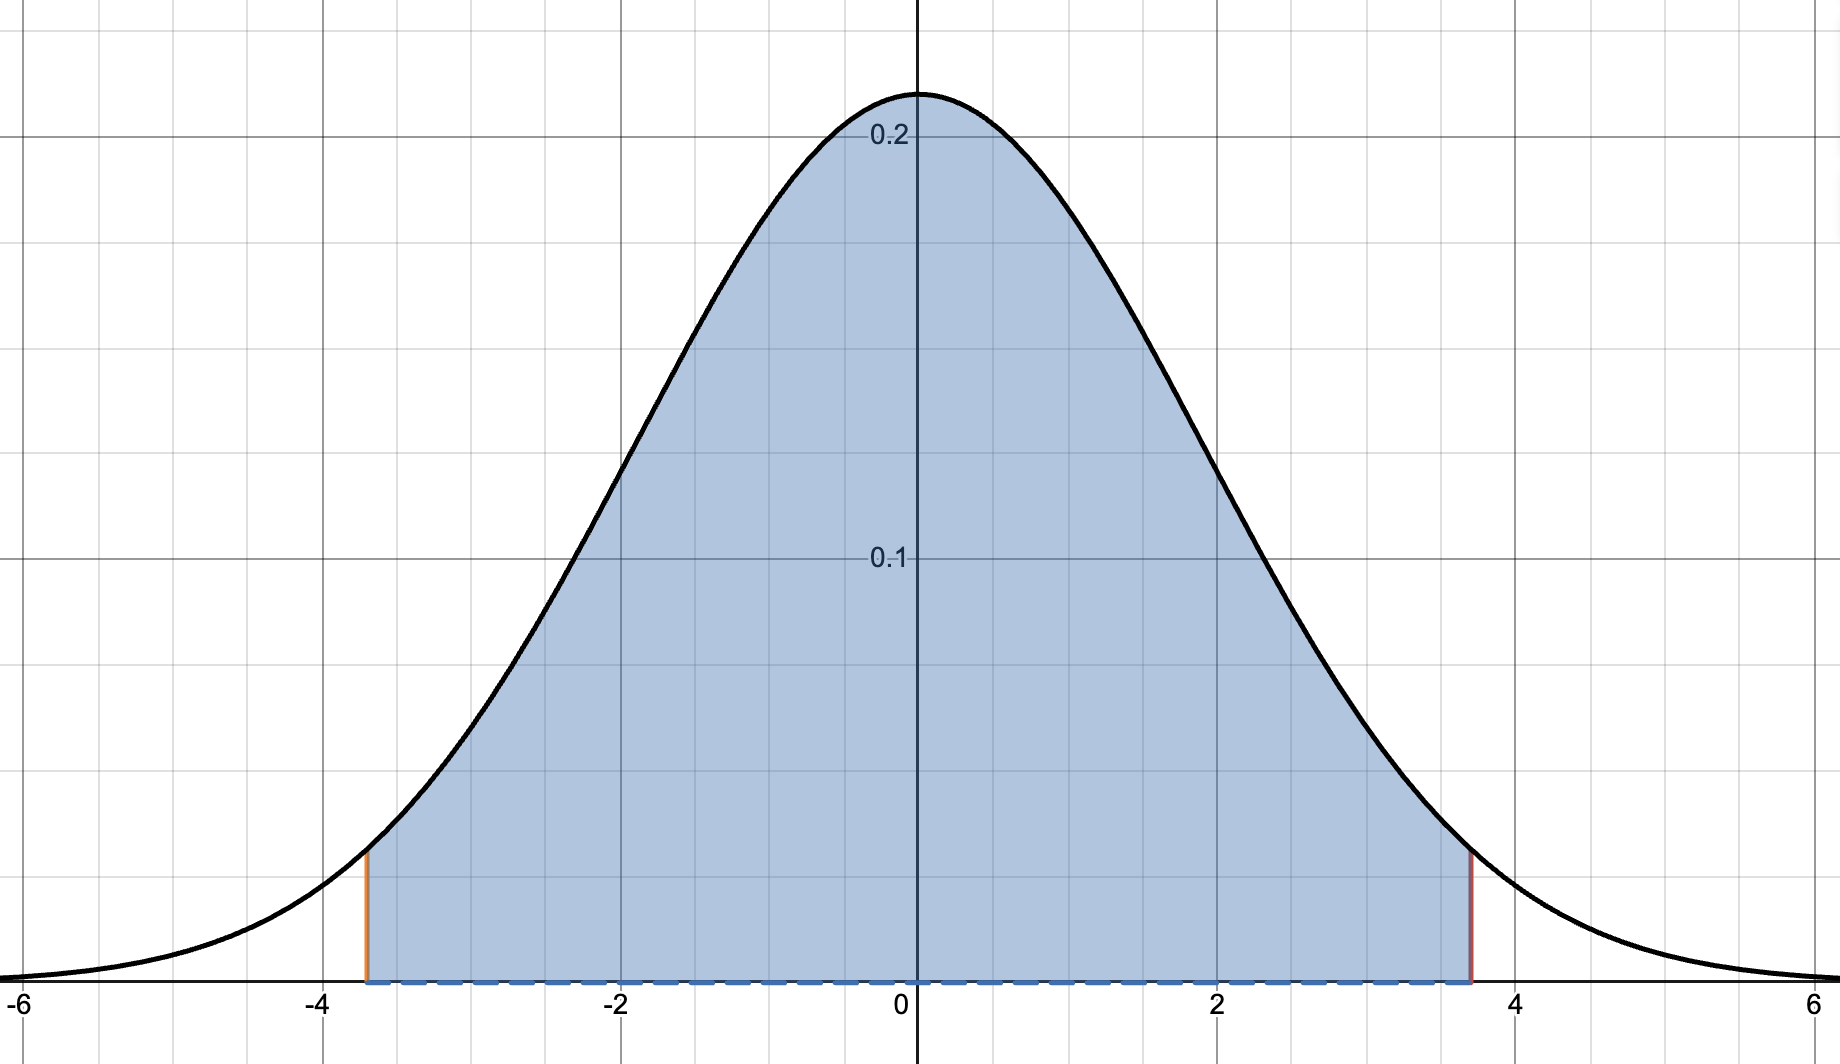
\includegraphics[width=0.5\textwidth]{normal.png}
            \end{center}
            et on repère les abscisses \(-t_\alpha\) et \(t_\alpha\) telles que l'aire bleue sous la courbe entre ces bornes vaut \(1-\alpha\).
        \end{solution}
    }{}
    \item Donner une valeur approchée pour $t_{0,05}, t_{0,01}$.
    \ifthenelse{\boolean{showSolutions}}{
        \begin{solution}
            On a \(t_{0,05}\mathop{\sim}1.96\) et \(t_{0,01}\mathop{\sim}2.58\).
        \end{solution}
    }{}

    \vspace{1em}
    Dans une population, un caractère est présent avec une proportion $p$. On cherche à estimer la valeur de $p$. 
    Pour cela, on étudie un échantillon de $n$ éléments de cette population, et on désigne par $X_n$ le nombre de fois où ce caractère est retrouvé dans l'échantillon.
    
    \item Quelle est la loi de $X_n$ ?
    \ifthenelse{\boolean{showSolutions}}{
        \begin{solution}
            \(X_n\) suit une loi binomiale de paramètres \((n,p)\).
        \end{solution}
    }{}
    \item On pose $Z_n=\frac{X_n-n p}{\sqrt{n p(1-p)}}$. Quel théorème permet d'affirmer que pour tous réels $a<b$, on a
$$
P\Big(Z_n \in[a, b]\Big) \rightarrow \int_a^b \frac{1}{\sqrt{2 \pi}} e^{-t^2 / 2} d t
$$
\ifthenelse{\boolean{showSolutions}}{
    \begin{solution}
        Le théorème central limite.
    \end{solution}
}{}

    \item On fixe $\alpha \in] 0,1\left[\right.$, et on pose 
    \[
    I_n=\left[p-t_\alpha \frac{\sqrt{p(1-p)}}{\sqrt{n}} ; p+t_\alpha \frac{\sqrt{p(1-p)}}{\sqrt{n}}\right].
    \]
    Déduire des questions précédentes que $\lim _{n \rightarrow+\infty} P\left(X_n / n \in I_n\right)=1-\alpha$.
    \ifthenelse{\boolean{showSolutions}}{
        \begin{solution}
            D'après la question précédente, \[\lim_{n\to\infty}P(Z_n\in[-t_\alpha,t_\alpha])=1-\alpha,\] 
            
            ce qui équivaut à \[\lim_{n\to\infty}P(X_n/n\in I_n)=1-\alpha.\]
        \end{solution}
    }{}
    \item Montrer que quel que soit $p\in]0,1[$, 
    \[
    I_n \subset\left[p-\frac{t_\alpha}{2 \sqrt{n}} ; p+\frac{t_\alpha}{2 \sqrt{n}}\right].
    \]
    \ifthenelse{\boolean{showSolutions}}{
        \begin{solution}
            Comme \(p(1-p)\le\frac14\), on a \(\frac{\sqrt{p(1-p)}}{\sqrt{n}}\le\frac1{2\sqrt{n}}\), 
            donc les bornes de \(I_n\) sont dans l'intervalle donné.
        \end{solution}
    }{}
    \item En déduire un intervalle de confiance au niveau $1-\alpha$ pour $p$.
    \ifthenelse{\boolean{showSolutions}}{
        \begin{solution}
            $p$ appartient à l'intervalle \[\left[\frac{X_n}{n}-\frac{t_\alpha}{2\sqrt{n}};\,\frac{X_n}{n}+\frac{t_\alpha}{2\sqrt{n}}\right]\] avec une probabilité de $1-\alpha$.
        \end{solution}
    }{}

    \vspace{1em}

    \textbf{Application : }
    Lors d'une élection opposant 2 candidats, un sondage d'opinion réalisé sur un échantillon de 1000 personnes donne \(52\%\) des voix au candidat \(A\), et \(48\%\) au candidat \(B\).
    \item Donner un intervalle de confiance au niveau 0,95 des intentions de vote pour \(A\).
    \ifthenelse{\boolean{showSolutions}}{
        \begin{solution}
            Pour le candidat $A$, $\frac{X_n}{n}=0.52$ et $\frac{t_{0.05}}{2\sqrt{n}}=\frac{1.96}{2\sqrt{1000}}\mathop{\sim}0.031$.
            On en déduit l'intervalle de confiance : 
            \[
            \left[0.52-0.031, 0.52+0.031\right] \mathop{\sim} [0.489, 0.551].
            \]
        \end{solution}
    }{} 
    \item Combien de personnes suffirait-il d'interroger pour qu'il y ait moins de \(5\%\) de chances que \(B\) l'emporte, si \(A\) a recueilli \(52\%\) ?
    \ifthenelse{\boolean{showSolutions}}{
        \begin{solution}
            Il suffit que la borne gauche de l'intervalle de confiance soit supérieure à $0.5$.

            Cela arrive si $0.52 - \frac{1.96}{2\sqrt{n}}>0.5$, soit $n>\frac{1.96^2}{2^2\times 0.02^2}\mathop{\sim}2401$.
        \end{solution}
    }{}
\end{enumerate}

\vspace{1cm}
\begin{center}
    \begin{tabular}{|r|r@{\ }r@{\ }r@{\ }r@{\ }r@{\ }r@{\ }r@{\ }r@{\ }r@{\ }r@{\ }|}
    \hline
    \multicolumn{11}{|c|}{NORMAL CUMULATIVE DISTRIBUTION FUNCTION}\\
    \hline
    \hline
    $x$&0.00&0.01&0.02&0.03&0.04&0.05&0.06&0.07&0.08&0.09\\
    \hline
    0.0&0.5000&0.5040&0.5080&0.5120&0.5160&0.5199&0.5239&0.5279&0.5319&0.5359\\
    \hline
    0.1&0.5398&0.5438&0.5478&0.5517&0.5557&0.5596&0.5636&0.5675&0.5714&0.5753\\
    \hline
    0.2&0.5793&0.5832&0.5871&0.5910&0.5948&0.5987&0.6026&0.6064&0.6103&0.6141\\
    \hline
    0.3&0.6179&0.6217&0.6255&0.6293&0.6331&0.6368&0.6406&0.6443&0.6480&0.6517\\
    \hline
    0.4&0.6554&0.6591&0.6628&0.6664&0.6700&0.6736&0.6772&0.6808&0.6844&0.6879\\
    \hline
    0.5&0.6915&0.6950&0.6985&0.7019&0.7054&0.7088&0.7123&0.7157&0.7190&0.7224\\
    \hline
    0.6&0.7257&0.7291&0.7324&0.7357&0.7389&0.7422&0.7454&0.7486&0.7517&0.7549\\
    \hline
    0.7&0.7580&0.7611&0.7642&0.7673&0.7703&0.7734&0.7764&0.7794&0.7823&0.7852\\
    \hline
    0.8&0.7881&0.7910&0.7939&0.7967&0.7995&0.8023&0.8051&0.8078&0.8106&0.8133\\
    \hline
    0.9&0.8159&0.8186&0.8212&0.8238&0.8264&0.8289&0.8315&0.8340&0.8365&0.8389\\
    \hline
    1.0&0.8413&0.8438&0.8461&0.8485&0.8508&0.8531&0.8554&0.8577&0.8599&0.8621\\
    \hline
    1.1&0.8643&0.8665&0.8686&0.8708&0.8729&0.8749&0.8770&0.8790&0.8810&0.8830\\
    \hline
    1.2&0.8849&0.8869&0.8888&0.8907&0.8925&0.8944&0.8962&0.8980&0.8997&0.9015\\
    \hline
    1.3&0.9032&0.9049&0.9066&0.9082&0.9099&0.9115&0.9131&0.9147&0.9162&0.9177\\
    \hline
    1.4&0.9192&0.9207&0.9222&0.9236&0.9251&0.9265&0.9279&0.9292&0.9306&0.9319\\
    \hline
    1.5&0.9332&0.9345&0.9357&0.9370&0.9382&0.9394&0.9406&0.9418&0.9429&0.9441\\
    \hline
    1.6&0.9452&0.9463&0.9474&0.9484&0.9495&0.9505&0.9515&0.9525&0.9535&0.9545\\
    \hline
    1.7&0.9554&0.9564&0.9573&0.9582&0.9591&0.9599&0.9608&0.9616&0.9625&0.9633\\
    \hline
    1.8&0.9641&0.9649&0.9656&0.9664&0.9671&0.9678&0.9686&0.9693&0.9699&0.9706\\
    \hline
    1.9&0.9713&0.9719&0.9726&0.9732&0.9738&0.9744&0.9750&0.9756&0.9761&0.9767\\
    \hline
    2.0&0.9772&0.9778&0.9783&0.9788&0.9793&0.9798&0.9803&0.9808&0.9812&0.9817\\
    \hline
    2.1&0.9821&0.9826&0.9830&0.9834&0.9838&0.9842&0.9846&0.9850&0.9854&0.9857\\
    \hline
    2.2&0.9861&0.9864&0.9868&0.9871&0.9875&0.9878&0.9881&0.9884&0.9887&0.9890\\
    \hline
    2.3&0.9893&0.9896&0.9898&0.9901&0.9904&0.9906&0.9909&0.9911&0.9913&0.9916\\
    \hline
    2.4&0.9918&0.9920&0.9922&0.9925&0.9927&0.9929&0.9931&0.9932&0.9934&0.9936\\
    \hline
    2.5&0.9938&0.9940&0.9941&0.9943&0.9945&0.9946&0.9948&0.9949&0.9951&0.9952\\
    \hline
    2.6&0.9953&0.9955&0.9956&0.9957&0.9959&0.9960&0.9961&0.9962&0.9963&0.9964\\
    \hline
    2.7&0.9965&0.9966&0.9967&0.9968&0.9969&0.9970&0.9971&0.9972&0.9973&0.9974\\
    \hline
    2.8&0.9974&0.9975&0.9976&0.9977&0.9977&0.9978&0.9979&0.9979&0.9980&0.9981\\
    \hline
    2.9&0.9981&0.9982&0.9982&0.9983&0.9984&0.9984&0.9985&0.9985&0.9986&0.9986\\
    \hline
    3.0&0.9987&0.9987&0.9987&0.9988&0.9988&0.9989&0.9989&0.9989&0.9990&0.9990\\
    \hline
    3.1&0.9990&0.9991&0.9991&0.9991&0.9992&0.9992&0.9992&0.9992&0.9993&0.9993\\
    \hline
    3.2&0.9993&0.9993&0.9994&0.9994&0.9994&0.9994&0.9994&0.9995&0.9995&0.9995\\
    \hline
    3.3&0.9995&0.9995&0.9995&0.9996&0.9996&0.9996&0.9996&0.9996&0.9996&0.9997\\
    \hline
    3.4&0.9997&0.9997&0.9997&0.9997&0.9997&0.9997&0.9997&0.9997&0.9997&0.9998\\
    \hline
    3.5&0.9998&0.9998&0.9998&0.9998&0.9998&0.9998&0.9998&0.9998&0.9998&0.9998\\
    \hline
    3.6&0.9998&0.9999&0.9999&0.9999&0.9999&0.9999&0.9999&0.9999&0.9999&0.9999\\
    \hline
    3.7&0.9999&0.9999&0.9999&0.9999&0.9999&0.9999&0.9999&0.9999&0.9999&0.9999\\
    \hline
    3.8&0.9999&0.9999&0.9999&0.9999&0.9999&0.9999&0.9999&0.9999&0.9999&0.9999\\
    \hline
    3.9&1.0000&1.0000&1.0000&1.0000&1.0000&1.0000&1.0000&1.0000&1.0000&1.0000\\
    \hline
    \end{tabular}
    \end{center}
    
\end{document}